\section{Programs in relation to the OS and the kernel}

\subsection{Sub topics}

\begin{itemize}
	\item Processes and threads.
	\item Threading model.
	\item Process anatomy.
	\item Virtual memory.
	\item Threads being executed on CPU, the associated scheduler and cache.
\end{itemize}

\subsection{Curriculum}

\begin{itemize}
	\item Slides "Intro to OS's".
	\item Slides "Parallel programs, processes and threads".
	\item OLA: "Anatomy of a program in memory", Gustavo Duarte.
	\item OLA: "The free lunch is over".
	\item OLA: "Virtual memory", pages 131-141.
	\item OLA: " Introduction to operating systems".
	\item OLA: "Multithreading".
	\item Kerrisk: Ch. 3-3.4 - System programming concepts.
	\item Kerrisk: Ch. 29 - Threads: Introduction.
\end{itemize}

\subsection{Exercises}

\begin{itemize}
	\item Posix Threads.
\end{itemize}

\newpage

\subsection{Processes and threads}
\begin{itemize}
	\item En \textbf{process} er en instans af et program, som eksekveres.
	\item En \textbf{thread} er en del af eksekveringen, alle processer har mindst én thread.
\end{itemize}

\subsubsection*{Processes}
\begin{itemize}
	\item Har hver sit memory space.
	\item Process A kan ikke skrive i Process B's hukommelse.
	\item Kan kun kommunikere gennem IPC\footnote{Inter-Process Communication, mekanismer kontrolleret af OS.}
	\item Kan skabe andre processer som kan eksekvere det samme eller andre programmer.
\end{itemize}

\subsubsection*{Threads}
\begin{itemize}
	\item Alle tråde i en process deler hukommelse på heap'en.
	\item Alle tråde har hver sin stack og \todo{hvad vil program counter sige?}program counter.
	\item Kan fucke med hinanden
	\begin{itemize}
		\item Skal passe på at man ikke sletter de øvrige trådes data.
	\end{itemize}
	Tråde er forskellige fra processer selvom de deler flere egenskaber og kendetegn. En tråd eksekveres i en process
\end{itemize}

\subsection{Threading model}
Der findes tre forskellige modeller:

\begin{itemize}
	\item User level threading.
	\item Kernel level threading.
	\item Hybrid level threading.
\end{itemize}

\subsubsection*{User level threading}
\begin{itemize}
	\item Simpel implementering, ingen kernel support for threads.
	\item Ekstremt hurtig thread kontekst skift (\todo{woot?}ikke brug for kernel handling).
	\item Ikke muligt at håndtere flere kerner\todo{hvorfor?}.
\end{itemize}

%\begin{figure}[H]
%	\centering
%	
\includegraphics{figs/userthreads}
%	\caption{User level threading illusteret.}
%	\label{fig:userthreads}
%\end{figure}

\subsubsection*{Kernel level threading}
\begin{itemize}
	\item Brug for thead bevisthed i kernel.
	\item Mapper direkte til threads som \textit{scheduleren} kan kontrollere.
	\item Effektiv brug af flere kerner.
\end{itemize}

%\begin{figure}[H]
%	\centering
%	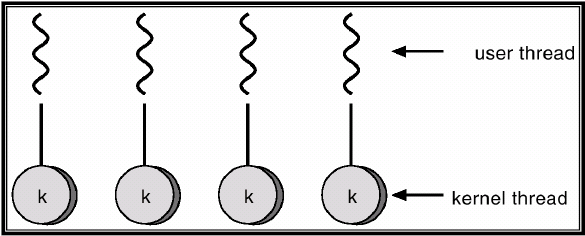
\includegraphics{figs/kernelthreads}
%	\caption{Kernel level threading illusteret.}
%	\label{fig:kernelthreads}
%\end{figure}

\subsubsection*{Hybrid level threading}
\begin{itemize}
	\item Komplex implementering\todo{why?}.
	\item Kræver god koordination mellem userspace og kernelspace scheduleren - ellers ikke optimal brug af resources.
\end{itemize}

%\begin{figure}[H]
%	\centering
%	
\includegraphics{figs/hybridthreads}
%	\caption{Hybrid level threading illusteret.}
%	\label{fig:hybridthreads}
%\end{figure}

\subsection{Process anatomy}
\begin{itemize}
	\item Når et program startes, starter en ny process.
	\item En process kører i sin egen memory sandbox, som et \textit{virtual address space} (4GB på 32-bit platform).
	\item Hver process har sin egen \textbf{pagetable/virtual address space}.
	\item Den virtuelle memory mapper til fysisk memory addresser vha. pagetables.
	\item Alle processer har \textbf{virtual address space}, hvor en del er bestemt til kernel space.
	\item Kernel space er ens for alle processor og mapper til samme fysiske hukommelse.
	\item Kernel space er flagged i pagetable med privileged code\todo{uddybning}, så kun kernel space programmer kan tilgå det memory. Page fault hvis user-space process forsøger at tilgå.
\end{itemize}

%\begin{figure}[H]
%	\centering
%	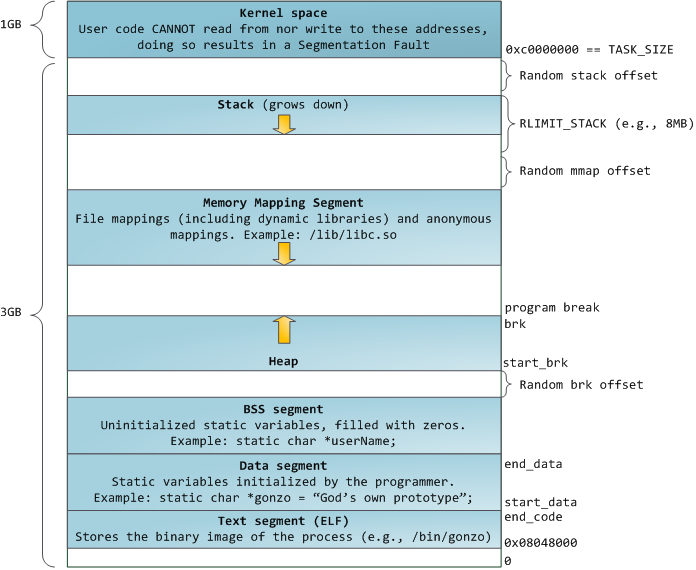
\includegraphics[width=\linewidth]{figs/memorydiagram}
%	\caption{Diagram over virtual address space allokering.}
%	\label{fig:memorydiagram}
%\end{figure}

Alle processors mapning ad virtual space er den samme. Af sikkerhedshensyn er der indført random-størrelse offsets mellem de forskellige enheder (stack, heap, etc.).\todo{bedre forklaring}\\

Resten, udover kernel space processens egen.\\

Her findes: Stack, heap, memory mapping, BSS, data og text/code segment.

%\begin{figure}[H]
%	\centering
%	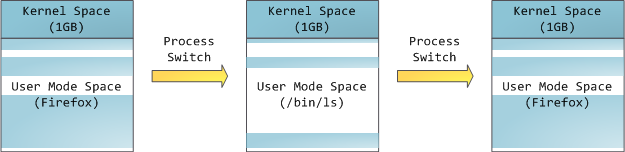
\includegraphics[width=\linewidth]{figs/memoryspace}
%	\caption{Diagram for process switch.}
%	\label{fig:memoryspace}
%\end{figure}

Alle processor har deres eget virtual address space, som bliver skiftet ved context switches, se figur~\ref{fig:memoryspace}. 

\paragraph{BSS}
Indeholder \textbf{ikke} initialiserede statiske variabler\todo{mere om dette?}. Dette område er anonymt\todo{udbyd!}.

\paragraph{Data segment}
Indeholder statisk initialiserede variabler, dette område er \textbf{ikke} anonymt, det er dog privat\todo{vil sige?}. Dette på kortlægger de initialiserede statiske værdier givet i source koden, fordi det er privat bliver ændringer ikke gemt i dette område\todo{igen, privat?}.\\

For eksempel, indholdet af en pointer er i data segmentet \todo{data og text segment??} men selve det den peger på ligger i \textbf{text segmentet}, som er \textit{read-only} og indeholder alt din kode \todo{min hvordan}. Text segmentet kortlægger ens binære filer i hukommelsen.

\subsection{Virtual memory}

\subsection{Threads being executed on CPU, associated scheduler and cache}







